\section{Forwards \& Futures in Practice}
\subsection*{2.1.1 US Treasury Bills}
\begin{itemize}
    \item \textbf{Dollar price}: Typically quoted per \$100 of face value
    \item Often given as \textbf{discount yield} $d$
    \[d=\frac{Par-P}{Par}\times\frac{360}{D}\]
    where $D$ is days to maturity.
    \item Dollar Price is then
    \[P=Par\times\left(1-d\times\frac{D}{360}\right)\]
    \item True yield is the \textbf{coupon equivalent yield} (CEY)
    or \textbf{investment rate}
\end{itemize}
\begin{enumerate}
    \item T-bills not more than half-year to maturity
    \[i=\frac{100-P}{P}\times\frac{y}{t}\]
    \item T-bills more than half-year to maturity. Root of
    \[\left(\frac{t}{2y}-0.25\right)i^2 + \frac{t}{y}i + \frac{P-100}{P}=0\]
\end{enumerate}

\subsection*{2.1.2 Accrued Interest}
\begin{center}
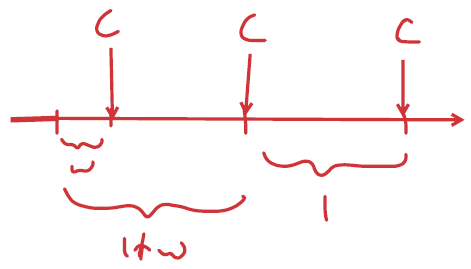
\includegraphics[width=0.3\linewidth]{contents/2.1.2.png}
\end{center}
Bond price a.k.a. \textbf{full, dirty, or invoice price}
\[P = \frac{F}{\left(1+\frac{r}{m}\right)^{w+n-1}}
+\sum_{i=0}^{n-1}\frac{C}{\left(1+\frac{r}{m}\right)^{w+i}}\]
Quoted prices a.k.a. \textbf{clean or flat price} 
does not include accrued interest.
\[DPrice=CPrice+AI\]

\subsection*{2.2.1 Repurchase Agreements}
\begin{itemize}
    \item Repurchase agreements = \textbf{repo} 
    = \textbf{collateralized loan}.
    \item Underlying security held as \textbf{collateral} 
    by counter-party.
    \item Counter-party entered \textbf{reverse repo}.
    \item Rate involved is \textbf{repo rate}.
    \item \textbf{Simple interest} rates. actual/360 in US.
\end{itemize}
\begin{center}
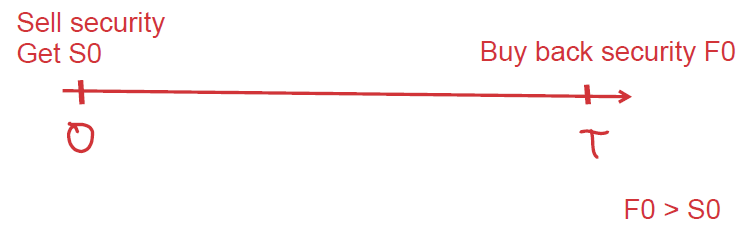
\includegraphics[width=0.5\linewidth]{contents/2.2.1.png}
\end{center}
\begin{enumerate}
    \item At time $t=0$, trader finances purchase of security worth $S_0$.
    \item Enter $T$-day repo with Mr. Y.
    \item Mr. Y demands haircut of $h\%$ and repo rate $r$.
    \item Mr. Y lends $S_0(1-h\%)$.
    \item Trader has net outflow of $S_0\times h\%$.
    \item At time $t=T$, trader pays $F=S_0(1-h\%)(1+r\times T/360)$.
    \item Trader receives security.
    \item Equivalent to forward purchase of security at forward price $F$.
    \item If security price increases to $S_T$ then trader earns profit.
    \item To carry out bet on decline using reverse repo, 
    buy at $S_0$, sell at $S_0(1-h\%)$, buy back at $S_T$.
\end{enumerate}

\subsection*{2.2.2 SOFR}
Secured Overnight Financing Rate (SOFR). Day count: actual/360.
Compound SOFR Formula
\[r=\left[\prod_{i=1}^{T}\left(1+\frac{r_i n_i}{Y}\right)-1\right]\frac{Y}{d_c}\]
Simple SOFR Formula
\[r=\frac{1}{d_c}\sum_{i=1}^T r_i n_i\]

\subsection*{2.2.3 1-Month and 3-Month SOFR Futures}
\begin{itemize}
    \item 1-month SOFR Futures: \$5m loan for 1-month
    \item 3-month SOFR Futures: \$1m loan for 3-months
    \item SOFR Futures follow 30 day periods
    \item Quoted Futures price 1-month: $100\times(1-E(r_m))$, 
    where $r_m$ is the simple average SOFR for contract month
    \item Final Settlement price 1-month: $100\times(1-r_m)$.
    \item Quoted Futures price 3-months: 
    $100\times(1-$ expected compound average SOFR for contract period)
\end{itemize}
\begin{itemize}
    \item Long position gains when expected SOFR falls (futures rises).
    \item Take up long position to hedge against rate falls.
    \item Long position is equivalent to agreeing to lend at rate 
    \[(100-F_0)\%\]
    \item Short position gains when expected SOFR rises (futures falls).
    \item Take up Short position to hedge against rate rises.
    \item Short position is equivalent to agreeing to borrow at rate 
    \[(100-F_0)\%\]
\end{itemize}
Changes to margin account
\begin{itemize}
    \item 1-month: Decrease in futures price by 0.01 (rate rise by 1 bp)
    results in long position being decreased by \$41.67.
    \item 3-months: Decrease in futures price by 0.01 (rate rise by 1 bp)
    results in long position being decreased by \$25.
\end{itemize}
\begin{center}
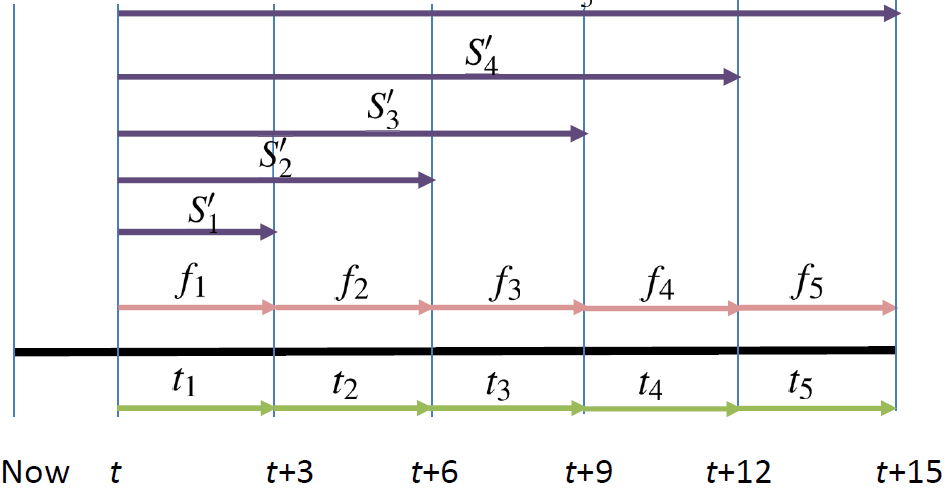
\includegraphics[width=0.6\linewidth]{contents/2.2.3.png}
\end{center}

\subsection*{2.2.4 Treasury Bond Futures}
Hypothetical 30-year 6\% (semi-annual) coupon bond w par value of \$100,000.
\[P_{inv} = N\times F_T \times CF + AI\]
Conversion Factor (CF) is clean price of \$1 coupon bond 
with maturity equal to deliverable bond if priced to yield 6\%.\\
With $n$ remaining coupon payments,
\[P=\frac{1}{1.03^{w+n-1}}+\sum_{i=0}^{n-1} \frac{c}{1.03^{w+i}}-c(1-w)\]
$w\in\{0.5,1\}$ is rounded to nearest quarter.\\
$CPrice$ is quoted bond price. $F_t$ is futures price.

Cheapest-to-Deliver (CTD)\\
$0$ is last coupon date, $t$ is till current date, 
$t+D$ until delivery, $T$ until next coupon
\[DPrice = CPrice + AI_t\]
\[AI_t = \frac{t}{T}\times \frac{c}{2}\times\$100\]
\[AI = \frac{t+D}{T}\times \frac{c}{2}\times\$100\]
Gross Basis
\[GB = CPrice - F_t \times CF\]
Net Basis
\[NB = DPrice \times (1+r\frac{D}{360})-(F_t\times CF + AI)\]
Implied Repo Rate (IRR)\\
rate of return from selling bond futures, then buying actual bond
\[IRR=\frac{(F_t\times CF + AI) - DPrice}{DPrice}\times \frac{360}{D}\]
\begin{center}
    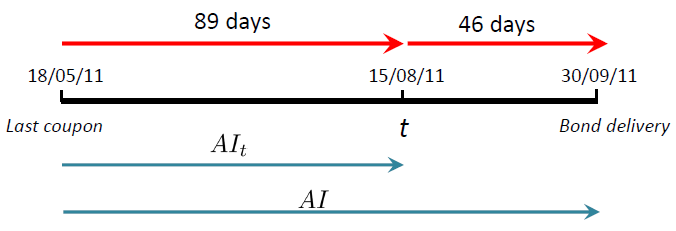
\includegraphics[width=0.6\linewidth]{contents/2.2.4.png}
\end{center}
\[t=89, D=46, T=185\]

\subsection*{2.2.5 Forward Rate Agreements (FRA)}
E.g. FRA covering period one month and ending four months is $1\times4$ contract.
Pricing FRAs, X is fixed rate (actual/360), y is actual ref rate (actual/360).
\[X = \left(\frac{d_{0,T}}{d_{0,T+m}}-1\right)\times\frac{360}{m}\]
Value of FRA
\[v=[d_{t,T} - \left(1+X\times\frac{m}{360}\right)\times d_{t,T+m}]\times N\]

\subsection*{2.3.1 Currency Prepaid Forward}
\[F_0^p=x_0 d_{0,T}(r_u)\]
for interest rate $r_u$, current exchange rate $x_0$.

\subsection*{2.3.2 Currency Forward}
\[F_0 = F_0^p / d_{0,T}(r_s)\]
Essentially the forward exchange rate.

\subsection*{2.3.3 Currency Futures}
FX futures convention: \textbf{base-currency/terms-currency}.